\documentclass{article}
\usepackage{graphicx} % Required for inserting images
\usepackage{multicol}
\usepackage[table]{xcolor}
\usepackage{colortbl}
\usepackage{geometry}
\usepackage{titlesec}
\geometry{a4paper, margin=1in}

% for custom headers
\usepackage{fancyhdr}
\pagestyle{fancy}
\fancyhf{}
\fancyhead[L]{\leftmark}
\fancyhead[R]{\thepage}
\renewcommand{\headrulewidth}{0.7pt}

% for custom table of contents
\usepackage{tocloft}
\setlength{\cftbeforesecskip}{0.6cm} % Adjust the value as needed


% Title spacing
\titlespacing*{\section}
{0pt}{3.5ex plus 1ex minus .2ex}{4.3ex plus .2ex}
\titlespacing*{\subsection}
{0pt}{3.25ex plus 1ex minus .2ex}{3.5ex plus .2ex}
\titlespacing*{\subsubsection}
{0pt}{3.25ex plus 1ex minus .2ex}{2.5ex plus .2ex}


\begin{document}

\begin{titlepage}


%TIKZ BACKGROUND
%\TITLEBOX

%CONTENT
\begin{center}

\sffamily
\textsc{\Huge\textcolor{black}{KSDSESM1KU}}\\[0.5cm]
\sffamily\textsc{\small{\textcolor{black}{DevOps, Software Evolution and Software Maintenance}}}\\[4cm]


% Upper part of the page. The '~' is needed because \\
% only works if a paragraph has started.

\includegraphics[width=0.5\textwidth]{images/ITU_logo_UK.jpg}~\\[3cm]


\includegraphics[width=0.2\textwidth]{images/llama.png}~\\[0.1cm]

{
 \huge \bfseries \sffamily Llama GeMsT \\[0.4cm] 
}

\normalfont \large \sffamily Project Report \\[2.5cm]


\noindent
\begin{minipage}{0.5\textwidth} % Adjusted to 0.5\textwidth for demonstration
\begin{flushleft} \large
\emph{Professors:} \\
Helge Pfeiffer - ropf@itu.dk \\
Mircea Lungu - mlun@itu.dk\\
\end{flushleft}
\end{minipage}%
\begin{minipage}{0.5\textwidth} % Adjusted to 0.5\textwidth for demonstration
\begin{flushright} \large
\emph{Authors:}\\
Simon Harwick – harw@itu.dk\\
Mihaela Hristova - mihr@itu.dk \\
Gustav Henrik Meding – gusm@itu.dk\\
Tomas Babkine-Di Caprio - tbab@itu.dk \\
Eduardo Sfreddo Trindade - edtr@itu.dk\\
\end{flushright}
\end{minipage}

\vfill

% Bottom of the page
\vfill
\vfill
{\large \today}

\end{center}
\end{titlepage}

\newpage
\tableofcontents
\newpage

\section{Introduction}
Th following report describes the work done during the Spring 2024 DevOps, Software Evolution and Software Maintenance taught at the IT University of Copenhagen. Our report includes the description of the final state of our system, the process we followed to develop and deploy it, lessons we learned, and reflections on technologies used and high and low level decisions we made throughout the semester.

\section{System's Perspective}
In this section, we describe the architecture of our Llama-MiniTwit system, the technologies that we used to support it, and we provide a rationale for the technologies we chose. This section also shows how a front-end or API request is processed by our system and what is eventually outputted. Finally, we show the results we obtained from using static analysis tools.

\subsection{Overall Architecture}
Figure \ref{fig:high_arch} is a visual representation of our overall architecture. We highlight its hierarchical nature starting from the hardware level on Digital Ocean to our services level installed on Docker containers. 
\begin{figure}
    \centering
    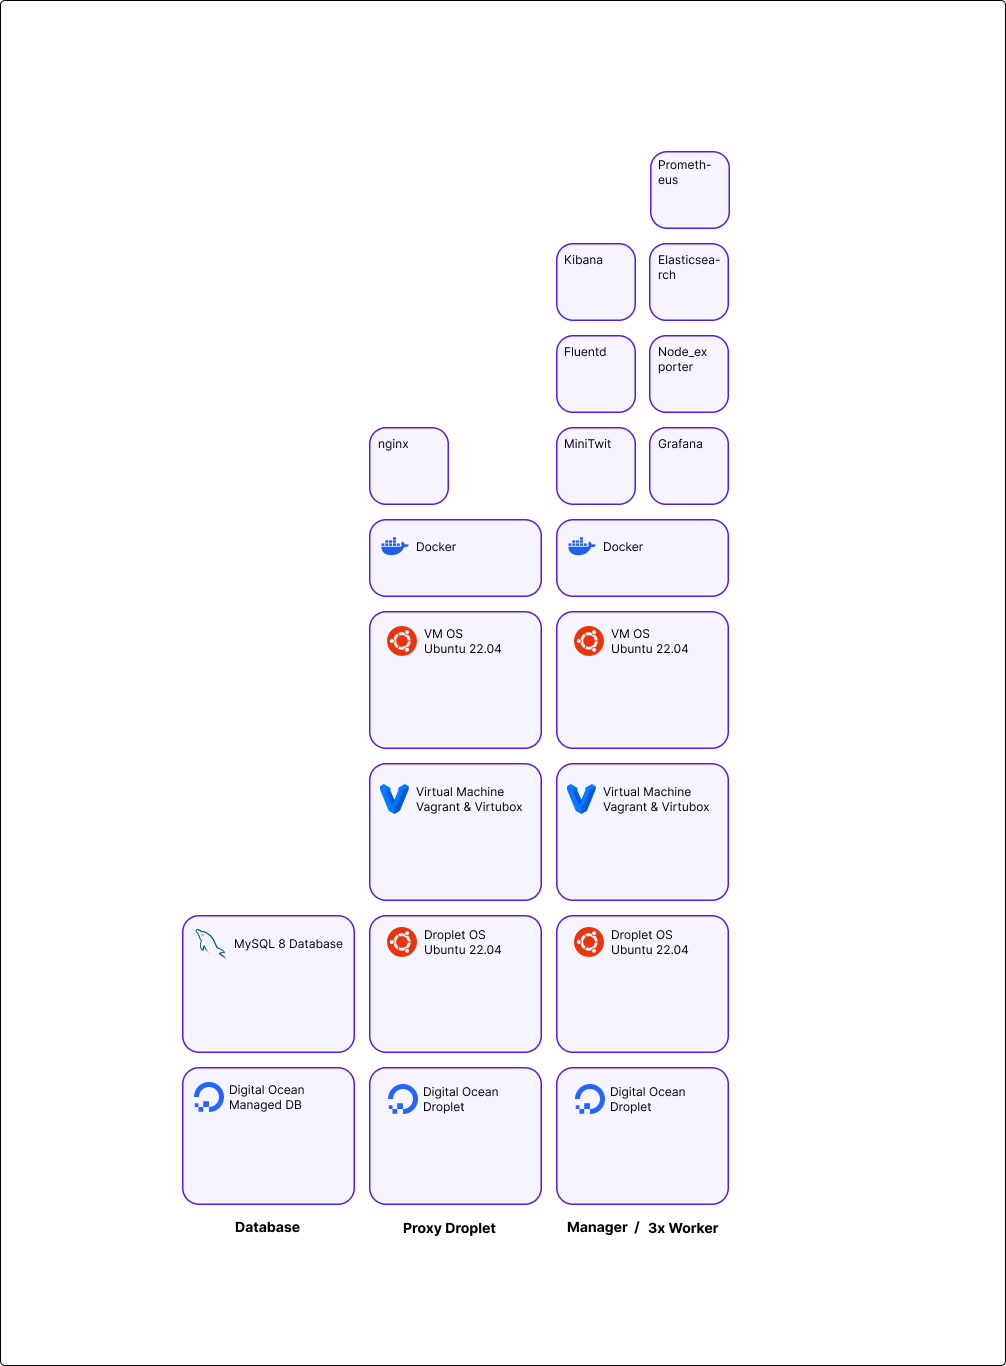
\includegraphics[width=1\linewidth]{./images/hierarchy.png}
    \caption{Hierarchical architecture mapping of our system.}
    \label{fig:high_arch}
\end{figure}

\subsection{Request Processing}
The diagram in figure \ref{fig:request_pipeline} shows how our system handles a request coming from the front-end or the API. We generally follow a model-view-controller architecture where the main function acts as the entry point of our application. Depending on the request type, the main function then forwards the request to handlers which redirect, handle logic, pass data to HTML templates or pass data to be written/read to/from the database. We chose this architecture as it would allow us to reuse code as much as possible and to seamlessly extend our code base. 
\\\\
For example, since we separated the methods that communicate with the database, we were able to add an abstraction layer without modifying the core logic of the application. Similarly, we were able to migrate our database from SQLite to a managed MySQL database on DigitalOcean very easily since our logic for connecting to the database was contained in one function which was invoked by several other function when they needed to connect to the database.

\begin{figure}[ht]
    \centering
    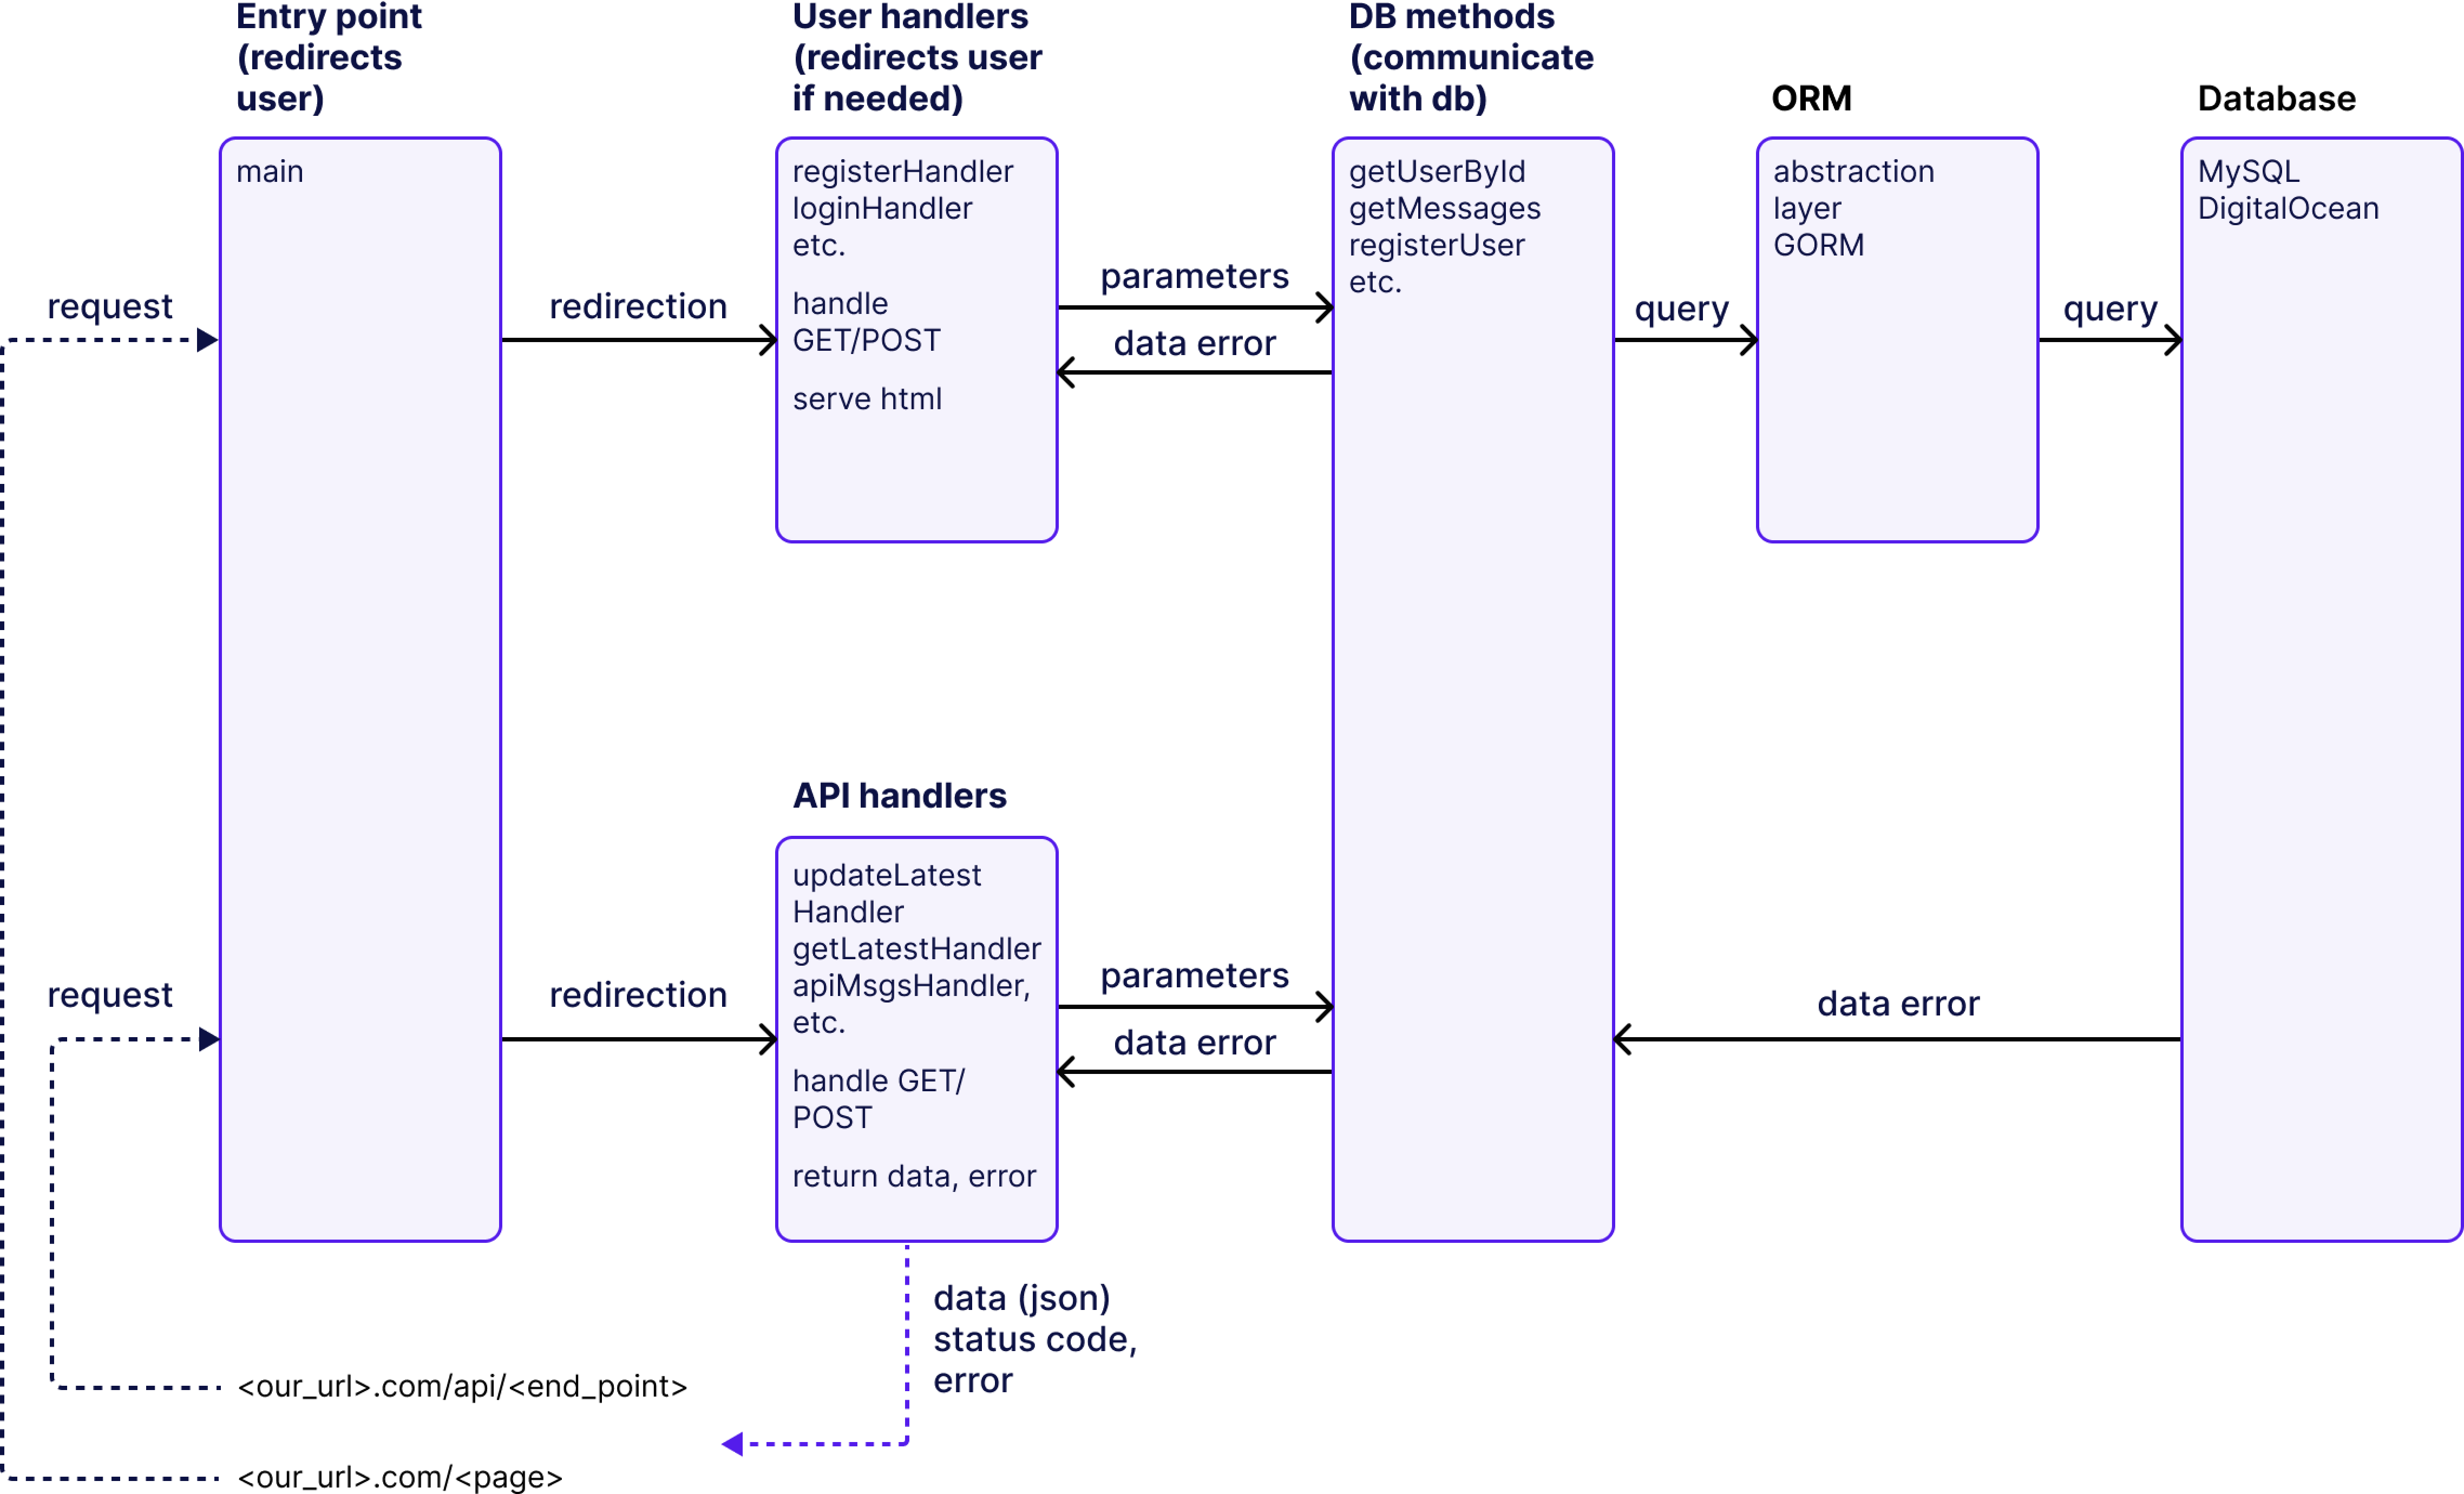
\includegraphics[width=1.0\textwidth]{./images/request_pipeline_v2.png}
    \caption{How our system handles a request.}
    \label{fig:request_pipeline}
\end{figure}

\subsection{Technologies used}
This section describes some of the key technologies used. The complete list of dependencies can be found in the appendix.

\subsubsection{Programming Languages}We chose to refactor our application using GoLang (Go). We chose to use it to refactor our app due to its simple syntax, automatic garbage collection and very high performance. Because of its easy to approach syntax, GoLang is generally regarded as a simple language to learn compared to others such as C++. For these reason, this made it a clear choice when we all saw the refactor of Llama-MiniTwit as an opportunity for us to learn a new language.
\\\\
The automated tests that were provided to us and that we used to monitor development on our app and make sure that no buggy code made it to our deployed application were written in Python. These were provided to us in the course repo and we chose not to refactor them to GoLang as we were able to use them to test our application in we received them.
\\\\
Finally, we used templated HTML files for the front-end of our application.

\subsubsection{Containerization and Orchestration Tools}
In order to ensure that our system had a high rate of availability (i.e., low downtime), we implemented a horizontal scaling strategy. While our cloud provider, Digital Ocean, allows for increasing droplet size through vertical scaling, we opted to also scale horizontally, thereby increasing availability through Docker Swarm. We selected this tool for three reasons:

\begin{enumerate}
    \item Ease of setup - since we already had experience with containerization Docker Swarm was easy to learn
    \item Load Balancing - Docker Swarm has built-in load-balancing thereby increasing performance
    \item Fault tolerance - by replicating nodes Docker Swarm increases fault tolerance and availability
\end{enumerate}

\subsubsection{Database Technologies}
We were first provided with a lightweight SQLite database for Llama-MiniTwit. While this worked well for some time, we eventually realized that we needed a more persistent form of storage. We chose to purchase DigitalOcean's managed MySQL database solution. This was an easy choice for us as we were already using DigitalOcean to deploy our app online. Furthermore, using one of their database solutions allowed us to automatically refuse any incoming connection, except if it originated from our application, which increased the security of our system greatly. We also chose their MySQL solution as it was very easy to duplicate the schema used in the SQLite database that was provided to us and because we would be storing very structured data, eliminating the need for a document based database.
\\\\
In addition to this, we implemented a database-abstraction-layer via GORM, an ORM library for GoLang. This was done for several reasons:

\begin{enumerate}
    \item Since GORM supports multiple databases like SQLite, MySQL and PostgreSQL this added flexibility to our system since we were not tied to one single database for the entire lifecycle of our system, and we could easily migrate if need be.
    \item GORM provides auto-migration, making it much easier to import an SQL table and perform operations on it. 
\end{enumerate}

\subsection{Static Analysis Tool Results}
We gave two static analysis tools access to our GitHub repository: SonarCloud and CodeClimate. Their outputs can be found in figures \ref{fig:sc_dashboard} and \ref{fig:cc_dashboard}. Both found some minor issues such as code smells, and maintainability issues, but did not raise any major problems such as bad code practices or security vulnerabilities. Furthermore, installing SonarCloud also gave us access to its bot which reviewed our code quality before we merged features into our main branch.

\begin{figure}[ht]
    \centering
    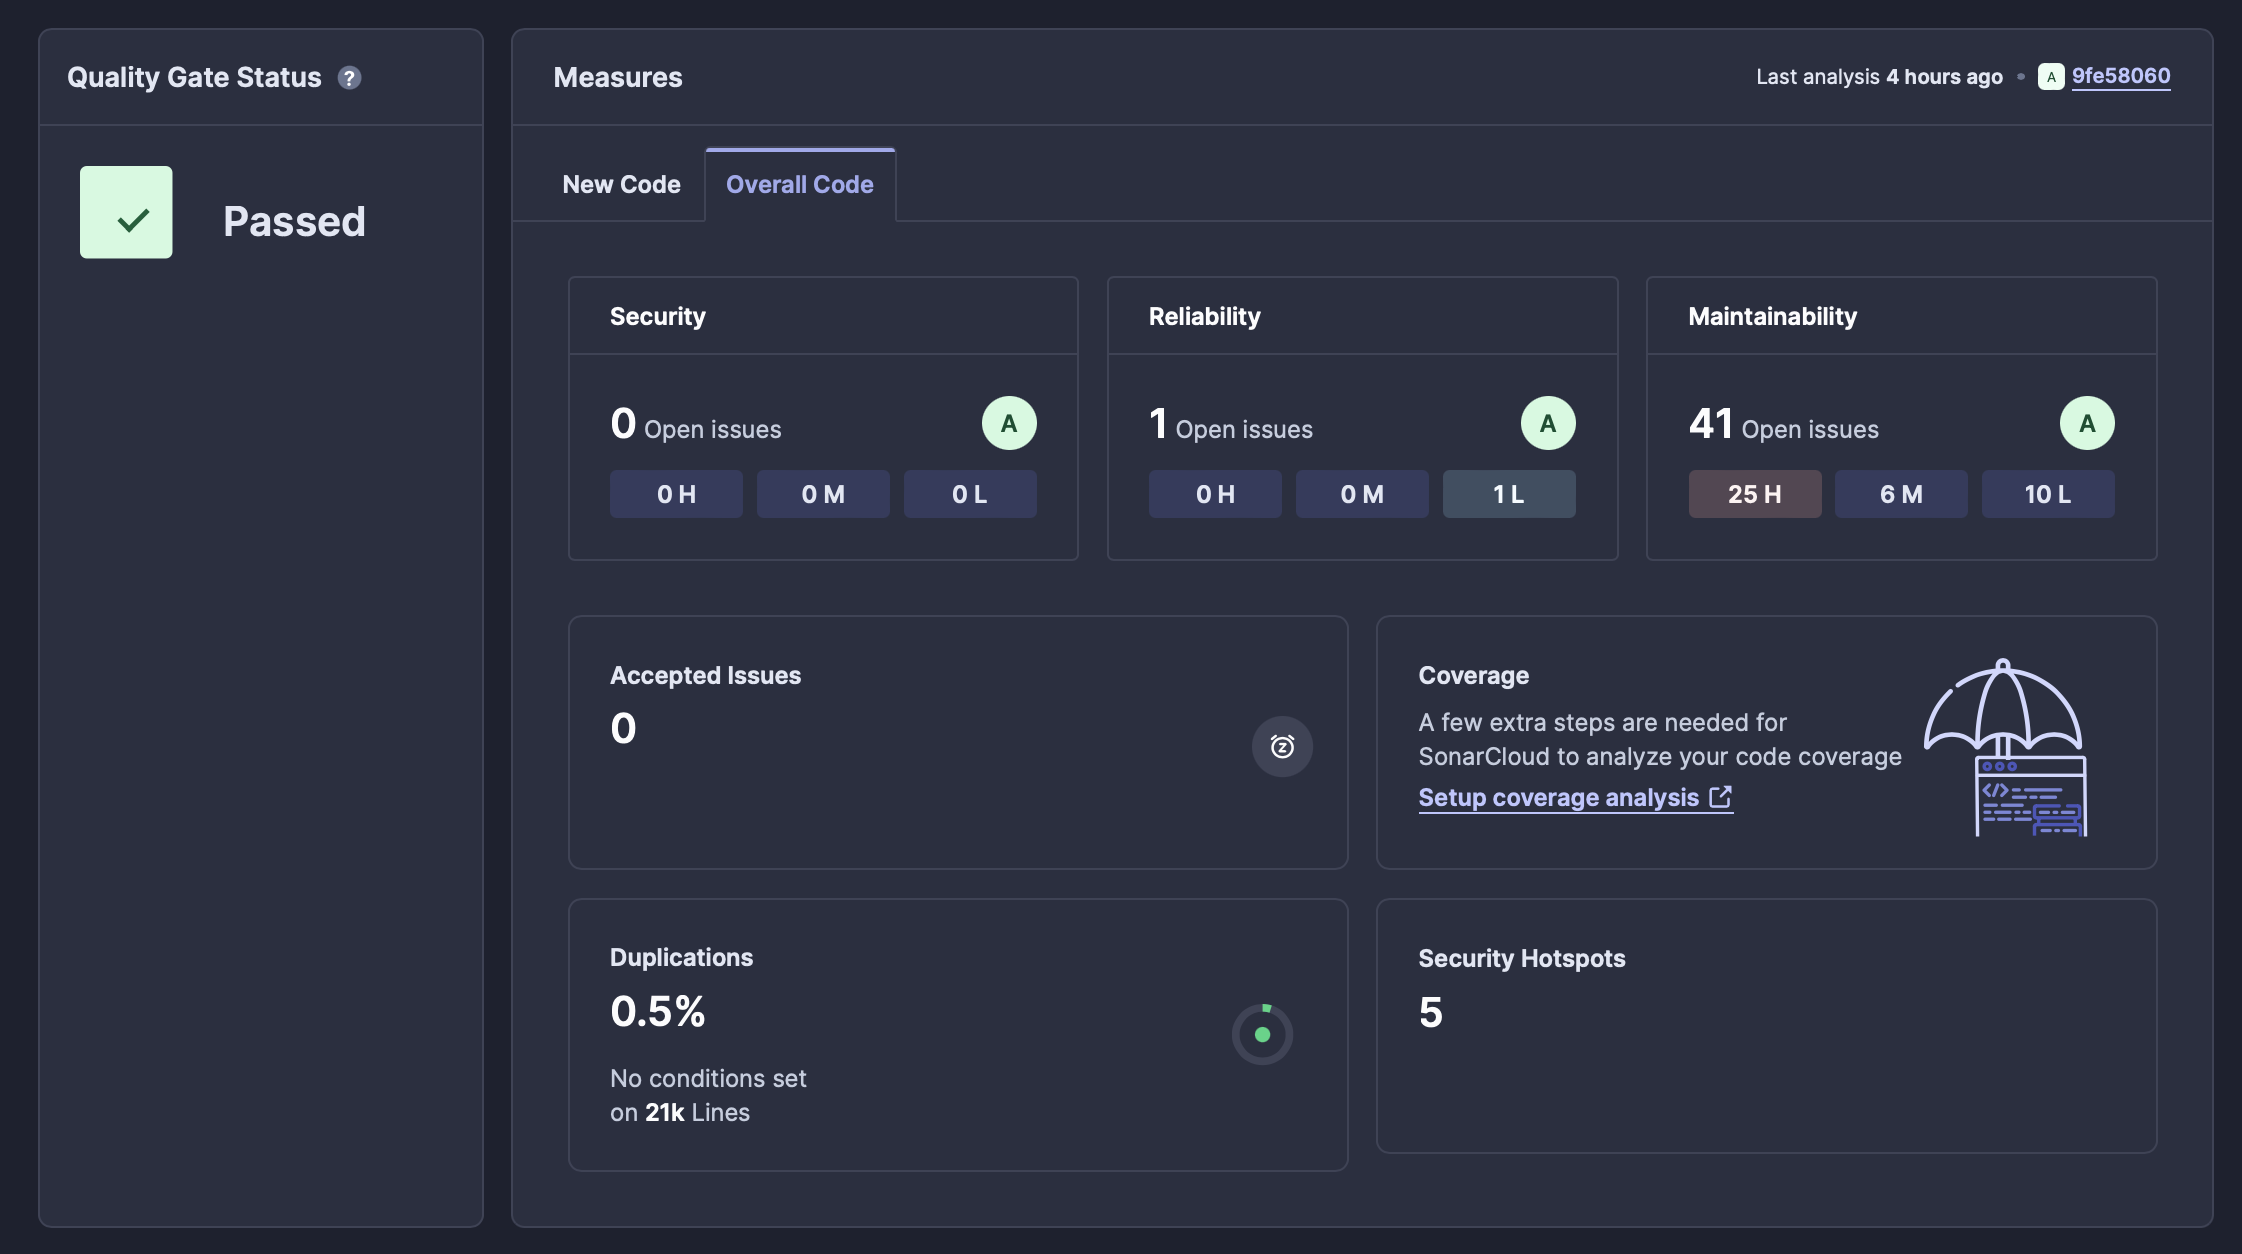
\includegraphics[width=0.8\textwidth]{./images/SonarCloud_Analysis.png}
    \caption{SonarCloud's dashboard after running an analysis on our repository.}
    \label{fig:sc_dashboard}
\end{figure}
\begin{figure}[ht]
    \centering
    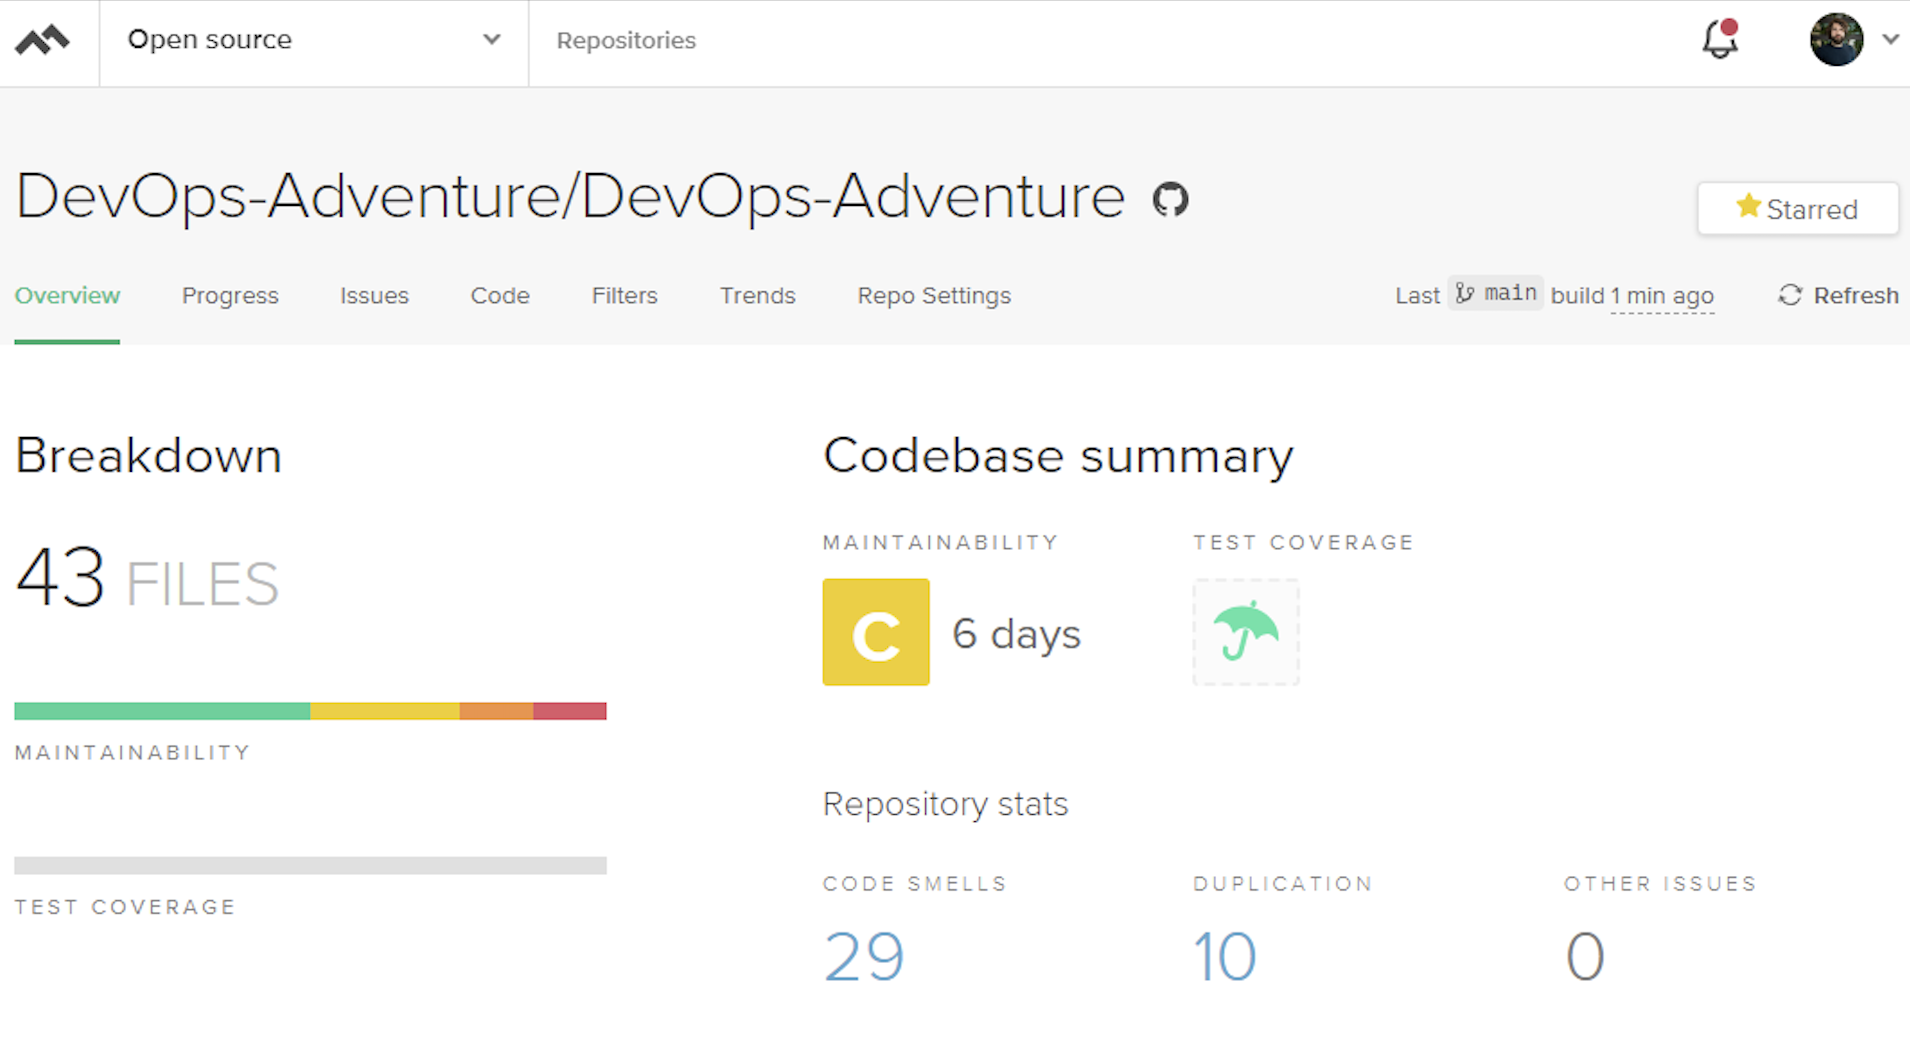
\includegraphics[width=0.8\textwidth]{./images/CodeClimate_analysis.png}
    \caption{Code Climate's dashboard after running an analysis on our repository.}
    \label{fig:cc_dashboard}
\end{figure}
\begin{figure}[ht]
    \centering
    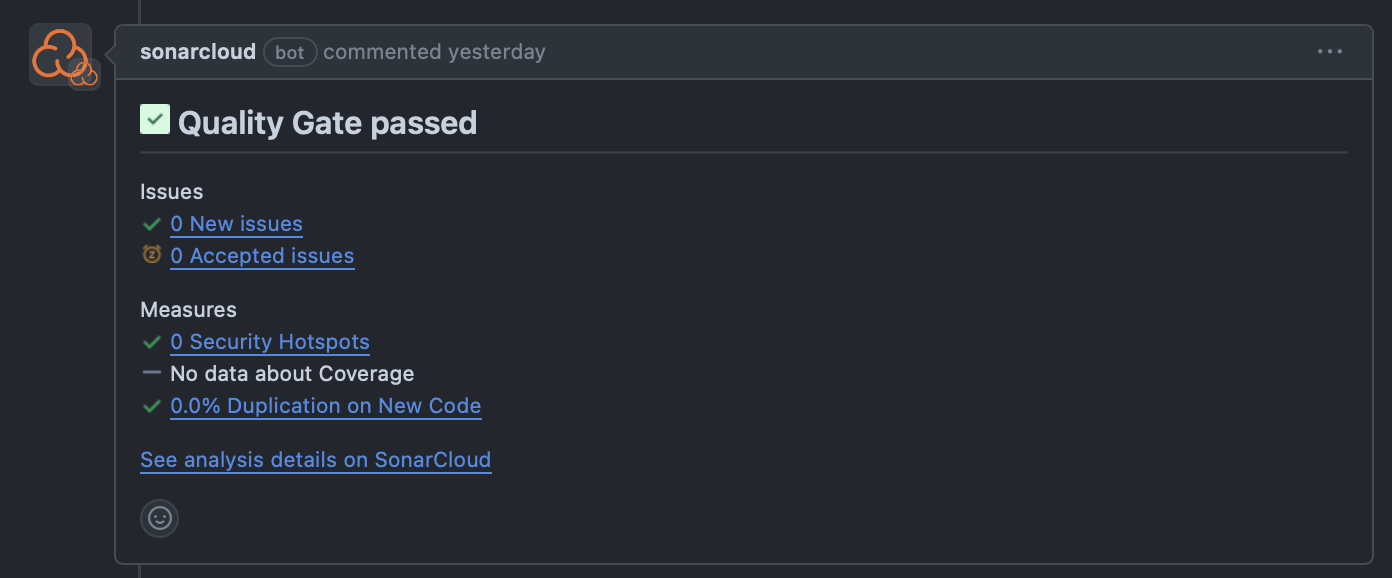
\includegraphics[width=0.8\textwidth]{./images/SonarCloud_bot.png}
    \caption{SonarCloud's bot adding comments on our pull requests.}
    \label{fig:sc_bot_dashboard}
\end{figure}
\pagebreak
\section{Process' Perspective}

\subsection{Initial Resource Partitioning}
Before deploying our system to DigitalOcean, we partitioned resources with the help of Vagrant.

\begin{figure}[ht]
    \centering
    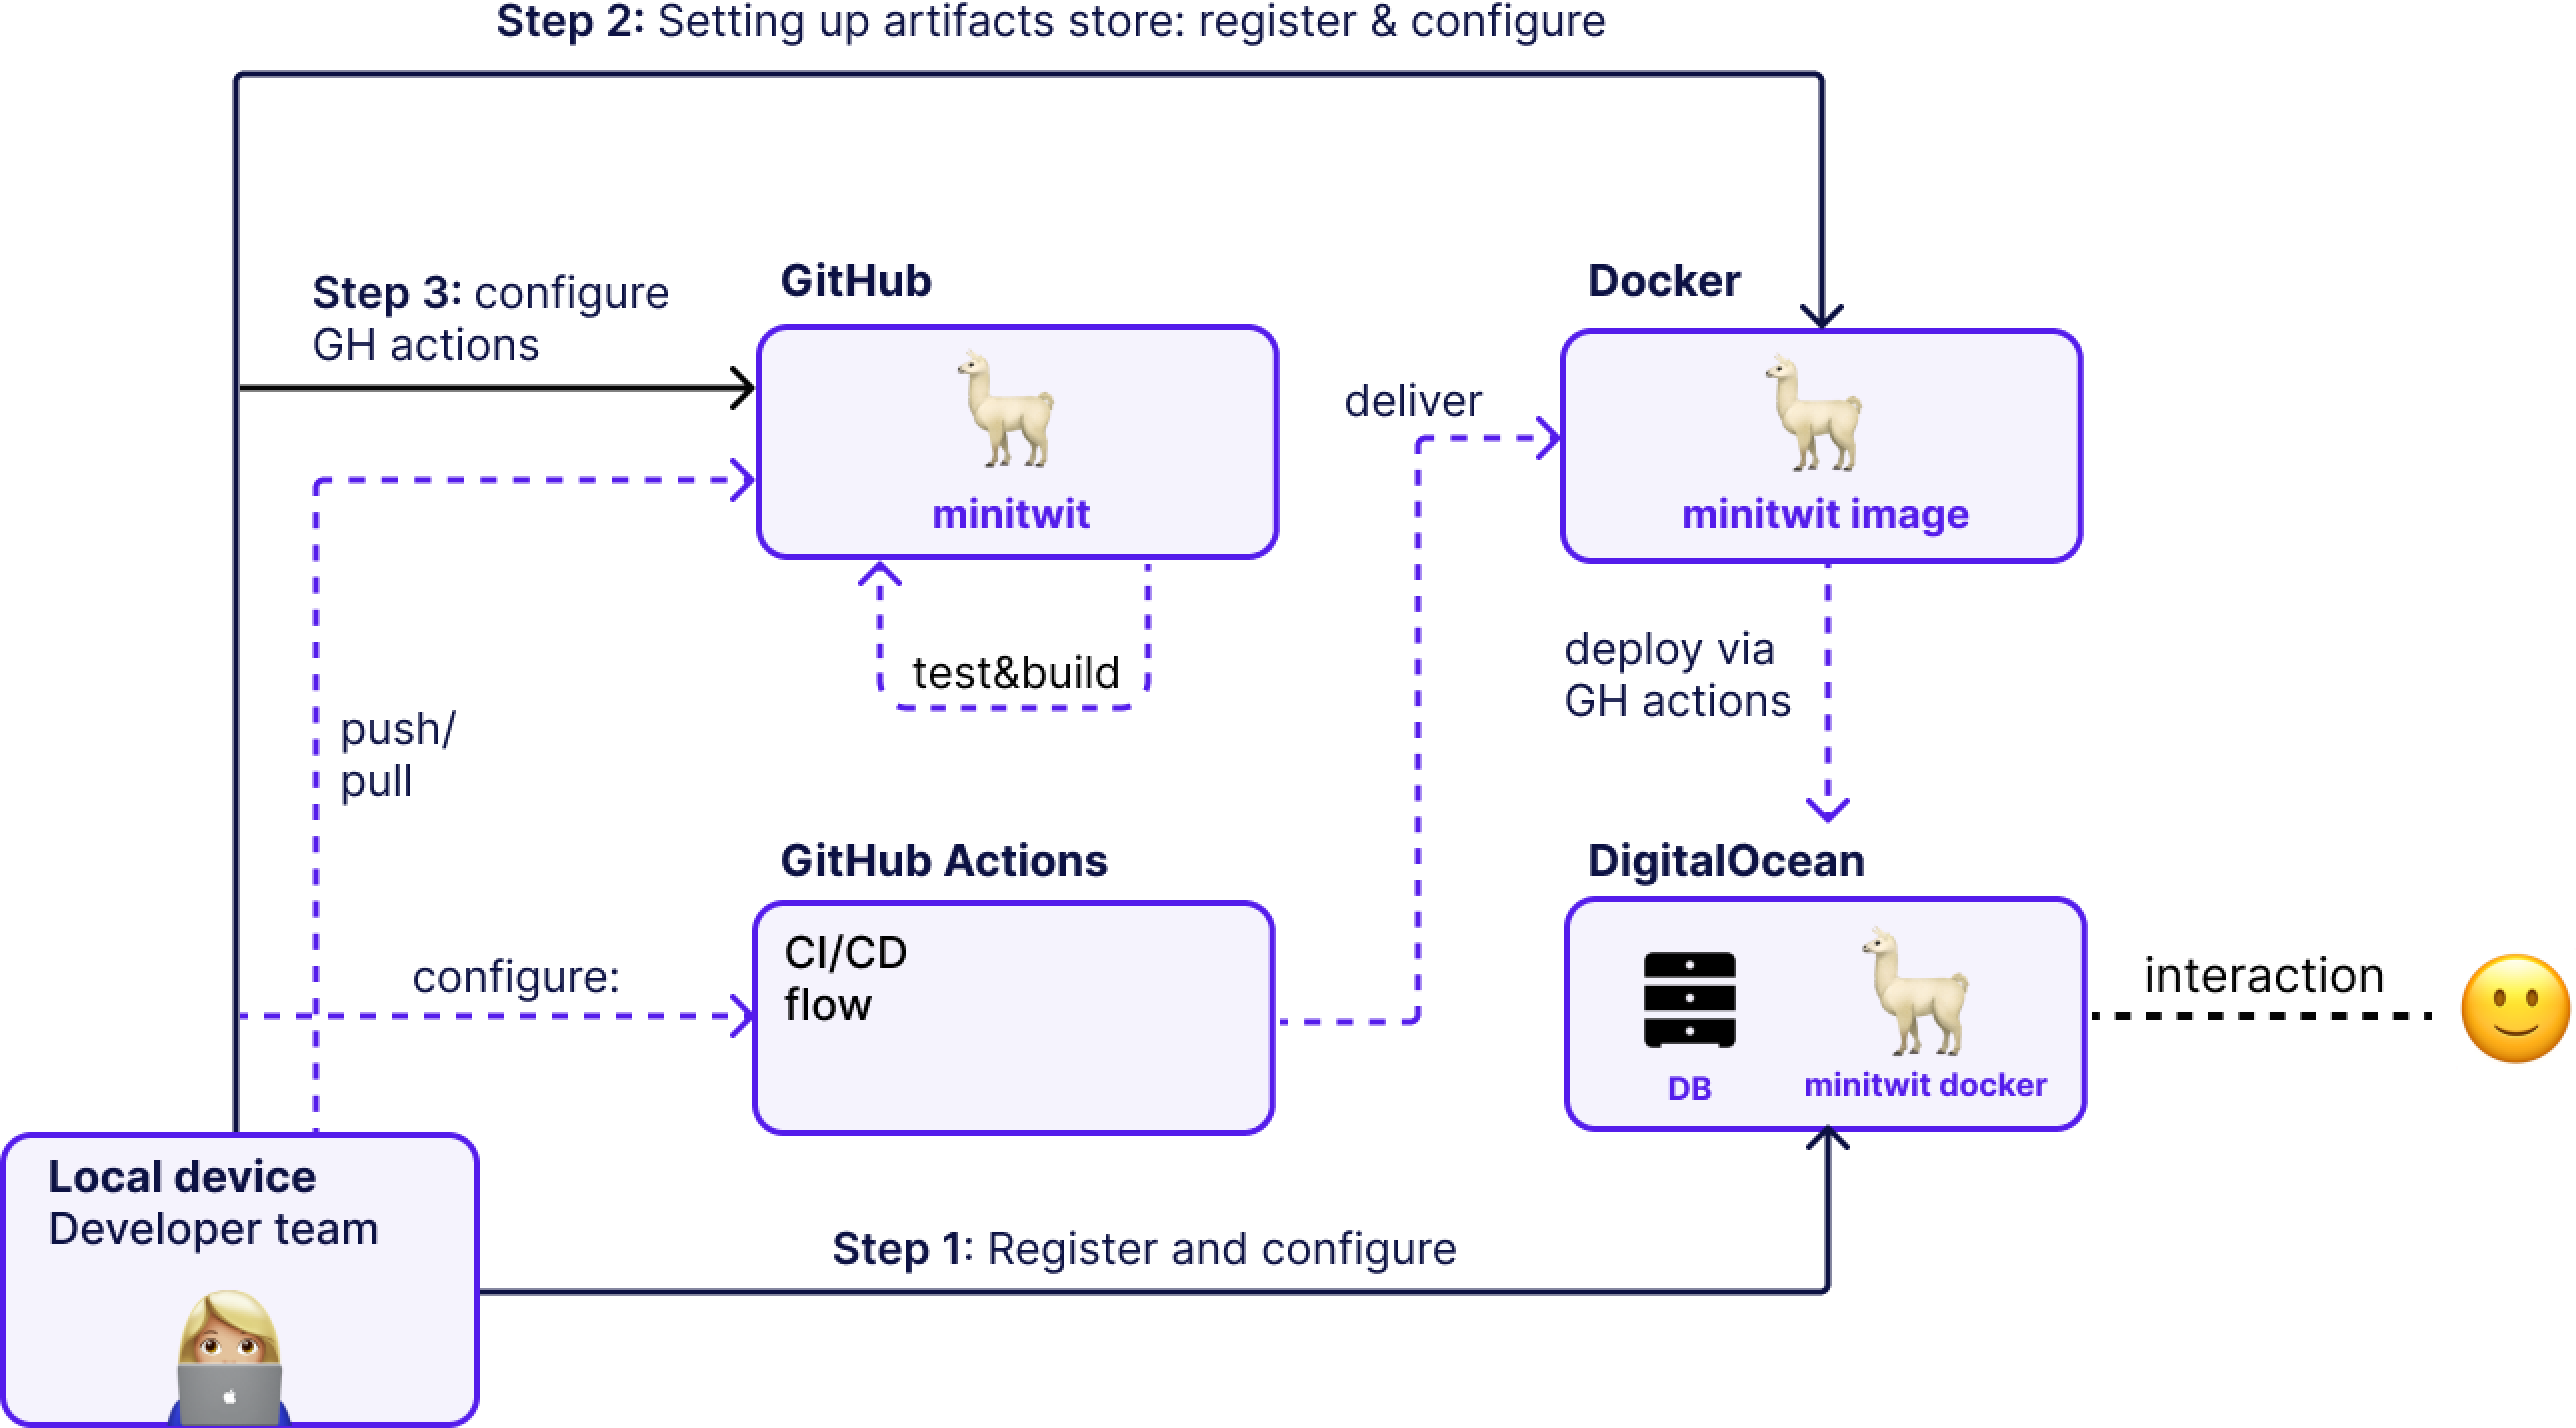
\includegraphics[width=0.8\textwidth]{./images/resources_setup_v2.png} 
    \caption{Resources setup for CI/CD pipeline.}
    \label{fig:Resourse setup}
\end{figure}

\subsubsection{Creation of the Virtual Machine and Server Setup on Digital Ocean}
We designed a Vagrant file to programatically create the droplet, start the virtual machine (VM), connect to the droplet, install Docker container and test that docker was functioning correctly.

\subsubsection{Setting Up Artifacts Store}
We registered in DockerHub to store our Llama-MiniTwit image and be able to easily push and pull changes from it. We also used DigitalOcean to deploy our app to a managed server, rather than manage a server ourselves to minimise maintenance and risk failure, ease of use and access, and multiple possibilities for integration for our system like Docker Swarm and hosting our database on the cloud. We chose DigitalOcean over other providers as the GitHub student developer pack gave us credits to use on the platform.

\subsubsection{Configuration of Secrets on our GitHub Repository}
We chose GitHub to store our codebase and to manage our CI/CD jobs. This required us to store secrets directly on the repository as environment variables so that they could be piped into our CI/CD actions. We also set up each member of our team with SSH key-pair access to the droplets to easily connect to the server.

\subsection{Development, Integration, Deployment {\&} Release}
\subsubsection{Development {\&} Pre-commit}
We utilized Git heavily during the course of this project. We also set up a few pre-commit hooks to facilitate development which would run linters such as golangci-lint, gofumpt and shellcheck. Finally, the pre-commit hooks also ran the tests that were provided to us.


\subsubsection{Continous Integration}
We created a continuous integration (CI) pipeline to enable us to test our code and new features frequently. We also created this pipeline to protect our main branch, where our Llama-MiniTwit was deployed, from having buggy or malicious code merged into it, as any merge into merge into main would automatically be deployed into our live system by our continuous deployment pipeline. Finally, we also setup our CI pipeline to run linters against code being added to the codebase, require pull requests to be reviewed and approved before they could be merged into our main branch and production environment. Figure \ref{fig:ci_pipeline} describes the steps in our CI pipeline and its main stages.

\begin{figure}[ht]
    \centering
    \includegraphics[width=1.0\textwidth]{./images/CI_pipline_V2.png} 
    \caption{Our continuous integration pipeline.}
    \label{fig:ci_pipeline}
\end{figure}

\subsection{Continuous Deployment}
We also established a continuous deployment (CD) pipeline to automatically deploy the updated version of our Llama-MiniTwit. Once a new feature was incorporated into the main branch of our repo after the successful merge of a pull request, our CD pipeline would automatically trigger and deploy the new version of our application. Our CD pipeline was executed with a GitHub action and had many responsibilities:

\begin{enumerate}
    \item Build the new version of Llama-MiniTwit and run tests against it.
    \item Build a new Docker image of our app and push it to DockerHub.
    \item Upload the deploy script from our repo to the DigitalOcean server
    \item Stop current containers running on the servers and download the new images from DockerHub.
    \item Start the containers with the new images.
    \item Release a new version of the Llama-MiniTwit on GitHub.
\end{enumerate}

If the CD pipeline successfully terminated, the new feature was deployed to our live system. It is important to note that the workers from the swarm were brought offline and back online using a rolling update scheme, to ensure that our system would always be available to access. This was easily implemented using Docker Swarm. The exact steps of the continuous deployment pipeline can be found in figure \ref{fig: cd_pipeline}.

\begin{figure}[ht]
    \centering
    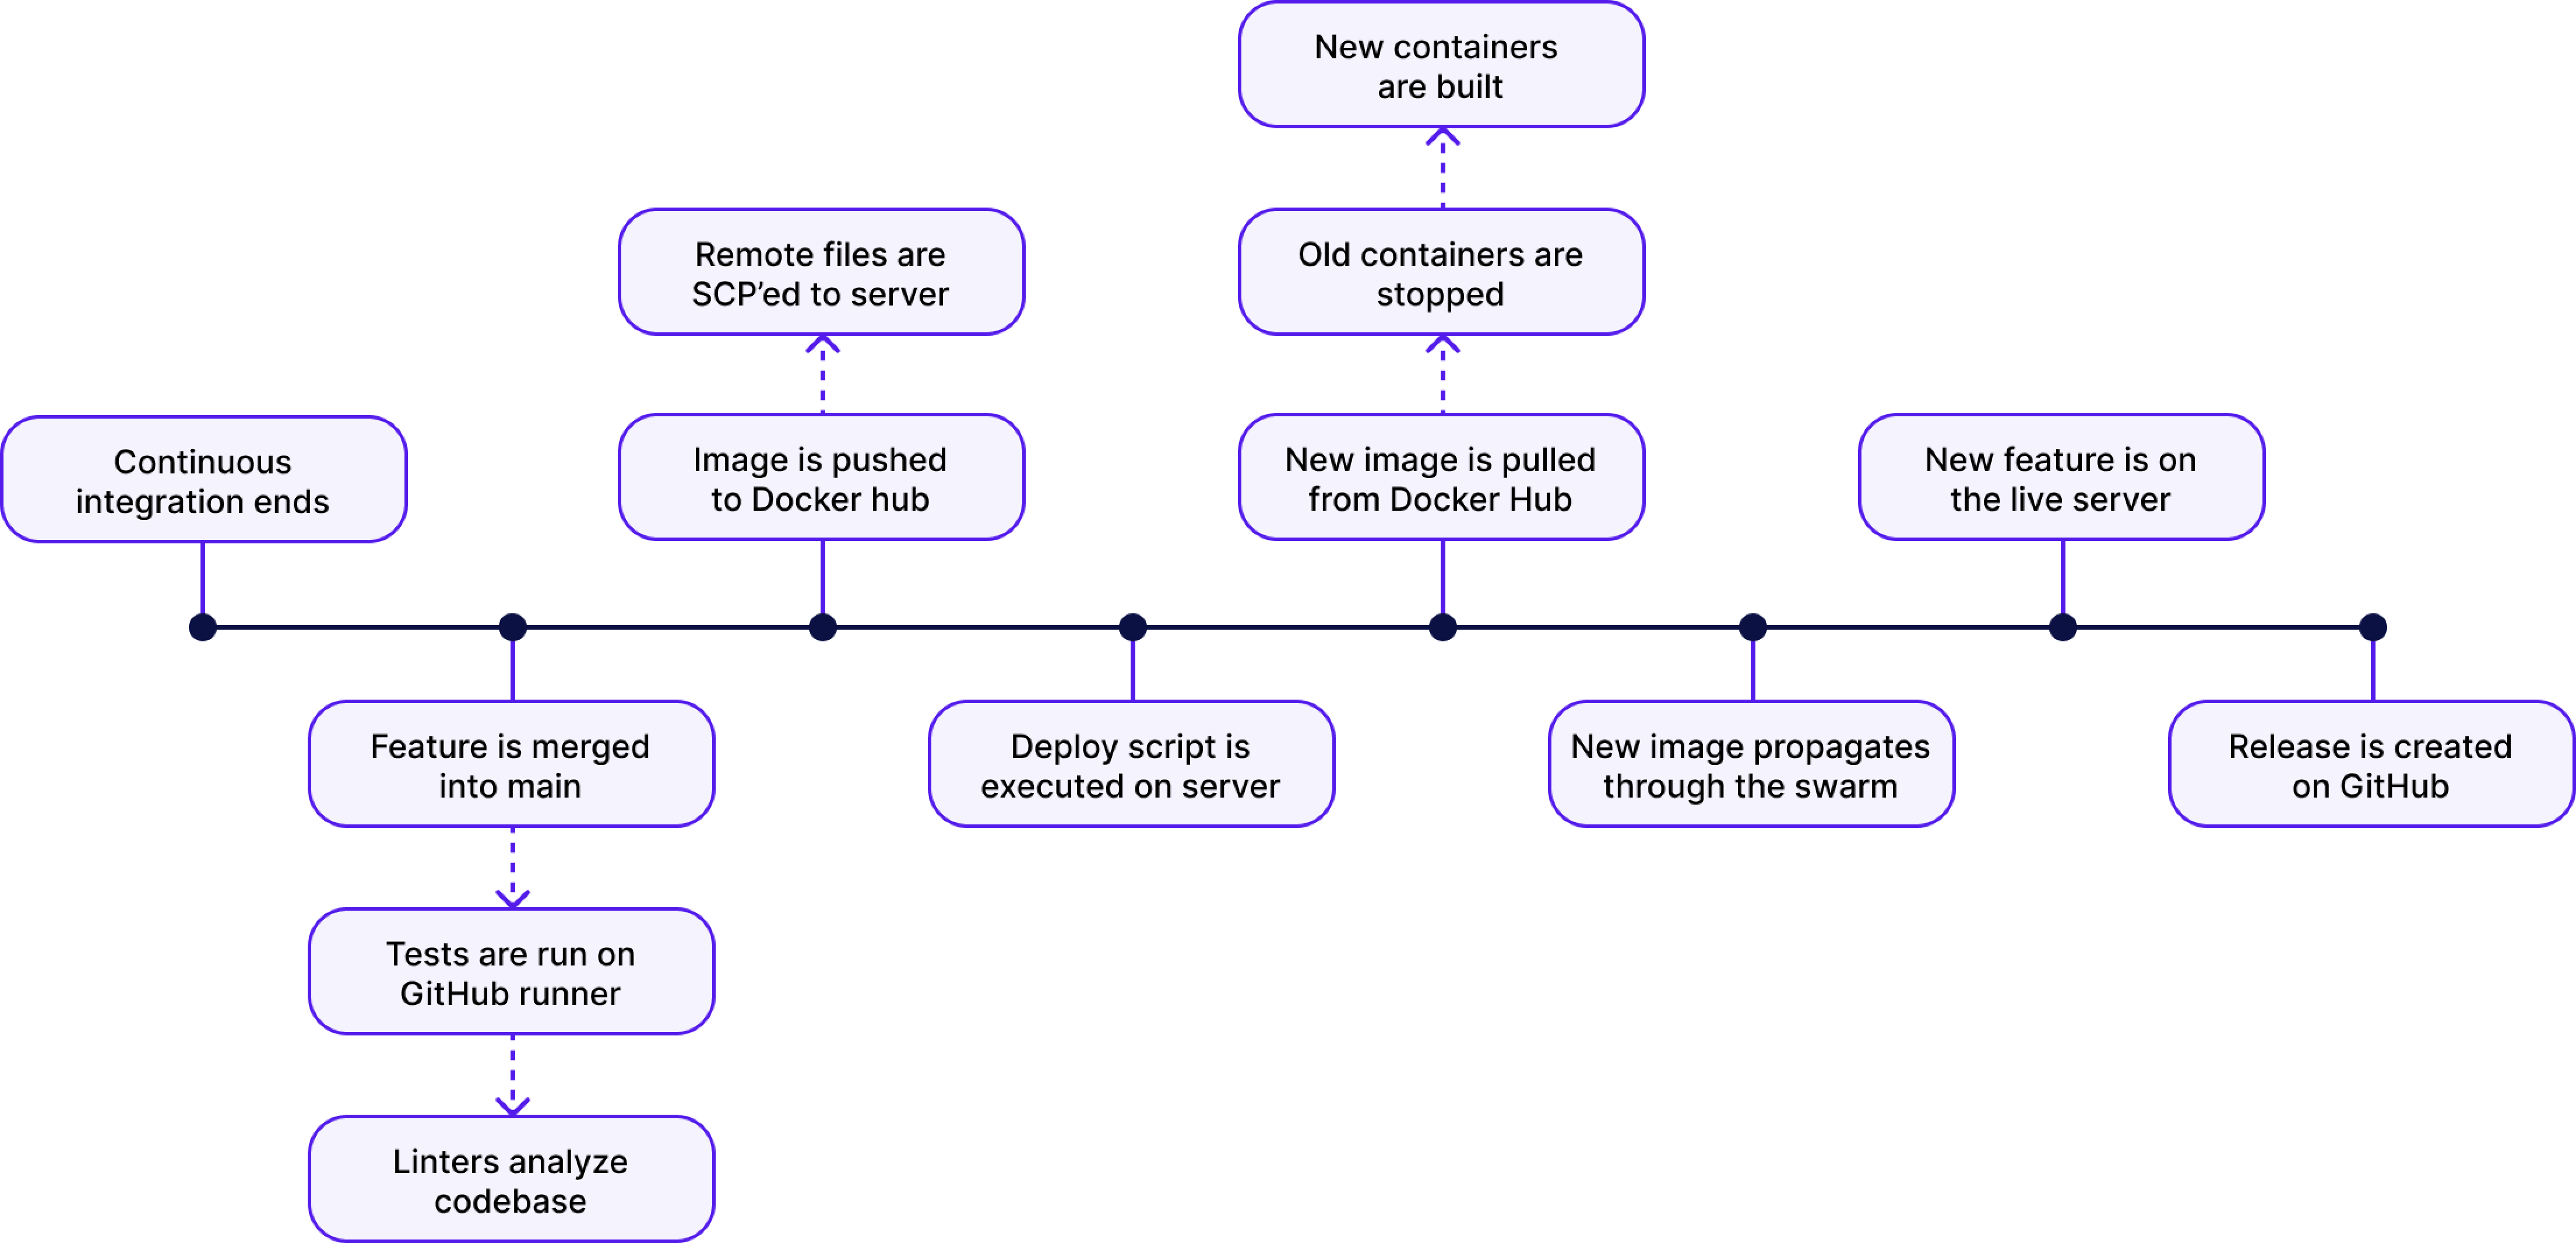
\includegraphics[width=1.0\textwidth]{./images/CD_pipeline_v2.png} 
    \caption{Our continuous deployment pipeline.}
    \label{fig: cd_pipeline}
\end{figure}

\subsection{Monitoring}

We used white box monitoring, which focuses on the processes within our application, providing insights for the internal state and performance of our application. We also used active monitoring, where we tracked interactions within our application, such as metrics for active logged users (note: without tracking their location).

\subsubsection{White Box Monitoring}

\begin{figure}[ht]
    \centering
    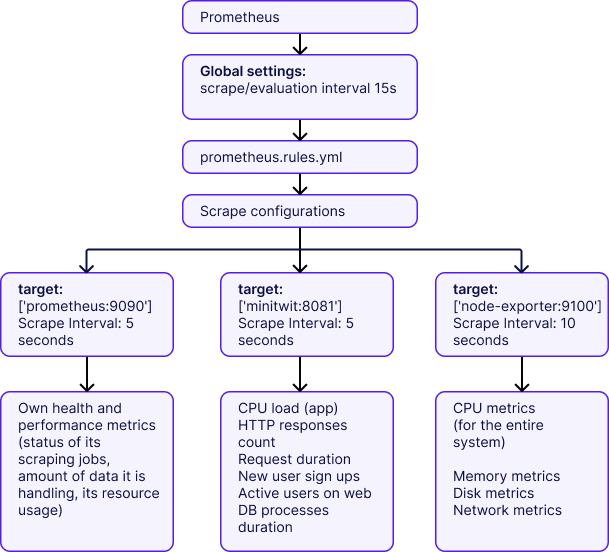
\includegraphics[width=0.6\textwidth]{./images/prometheus_configuration_v2.png} 
    \caption{Prometheus configuration.}
    \label{fig:prometheus_configuration}
\end{figure}

Figure \ref{fig:prometheus_configuration} depicts the configurations we chose for Prometheus, and how and where it collects information. We chose to monitor metrics on two levels: application and system level.

\begin{enumerate}
    \item CPU load in the application. A Grafana dashboard helped us diagnose a bug where the operating system of our virtual machine would starve our containers randomly.
    \item Monitoring CPU, Memory, and Network metrics in the hosting system helped us determine whether issues originate locally within the application or at the server level. It was of crucial important to be informed about overall health of the hosting environment as it could affect our application performance.
\end{enumerate}

\begin{figure}[ht]
    \centering
    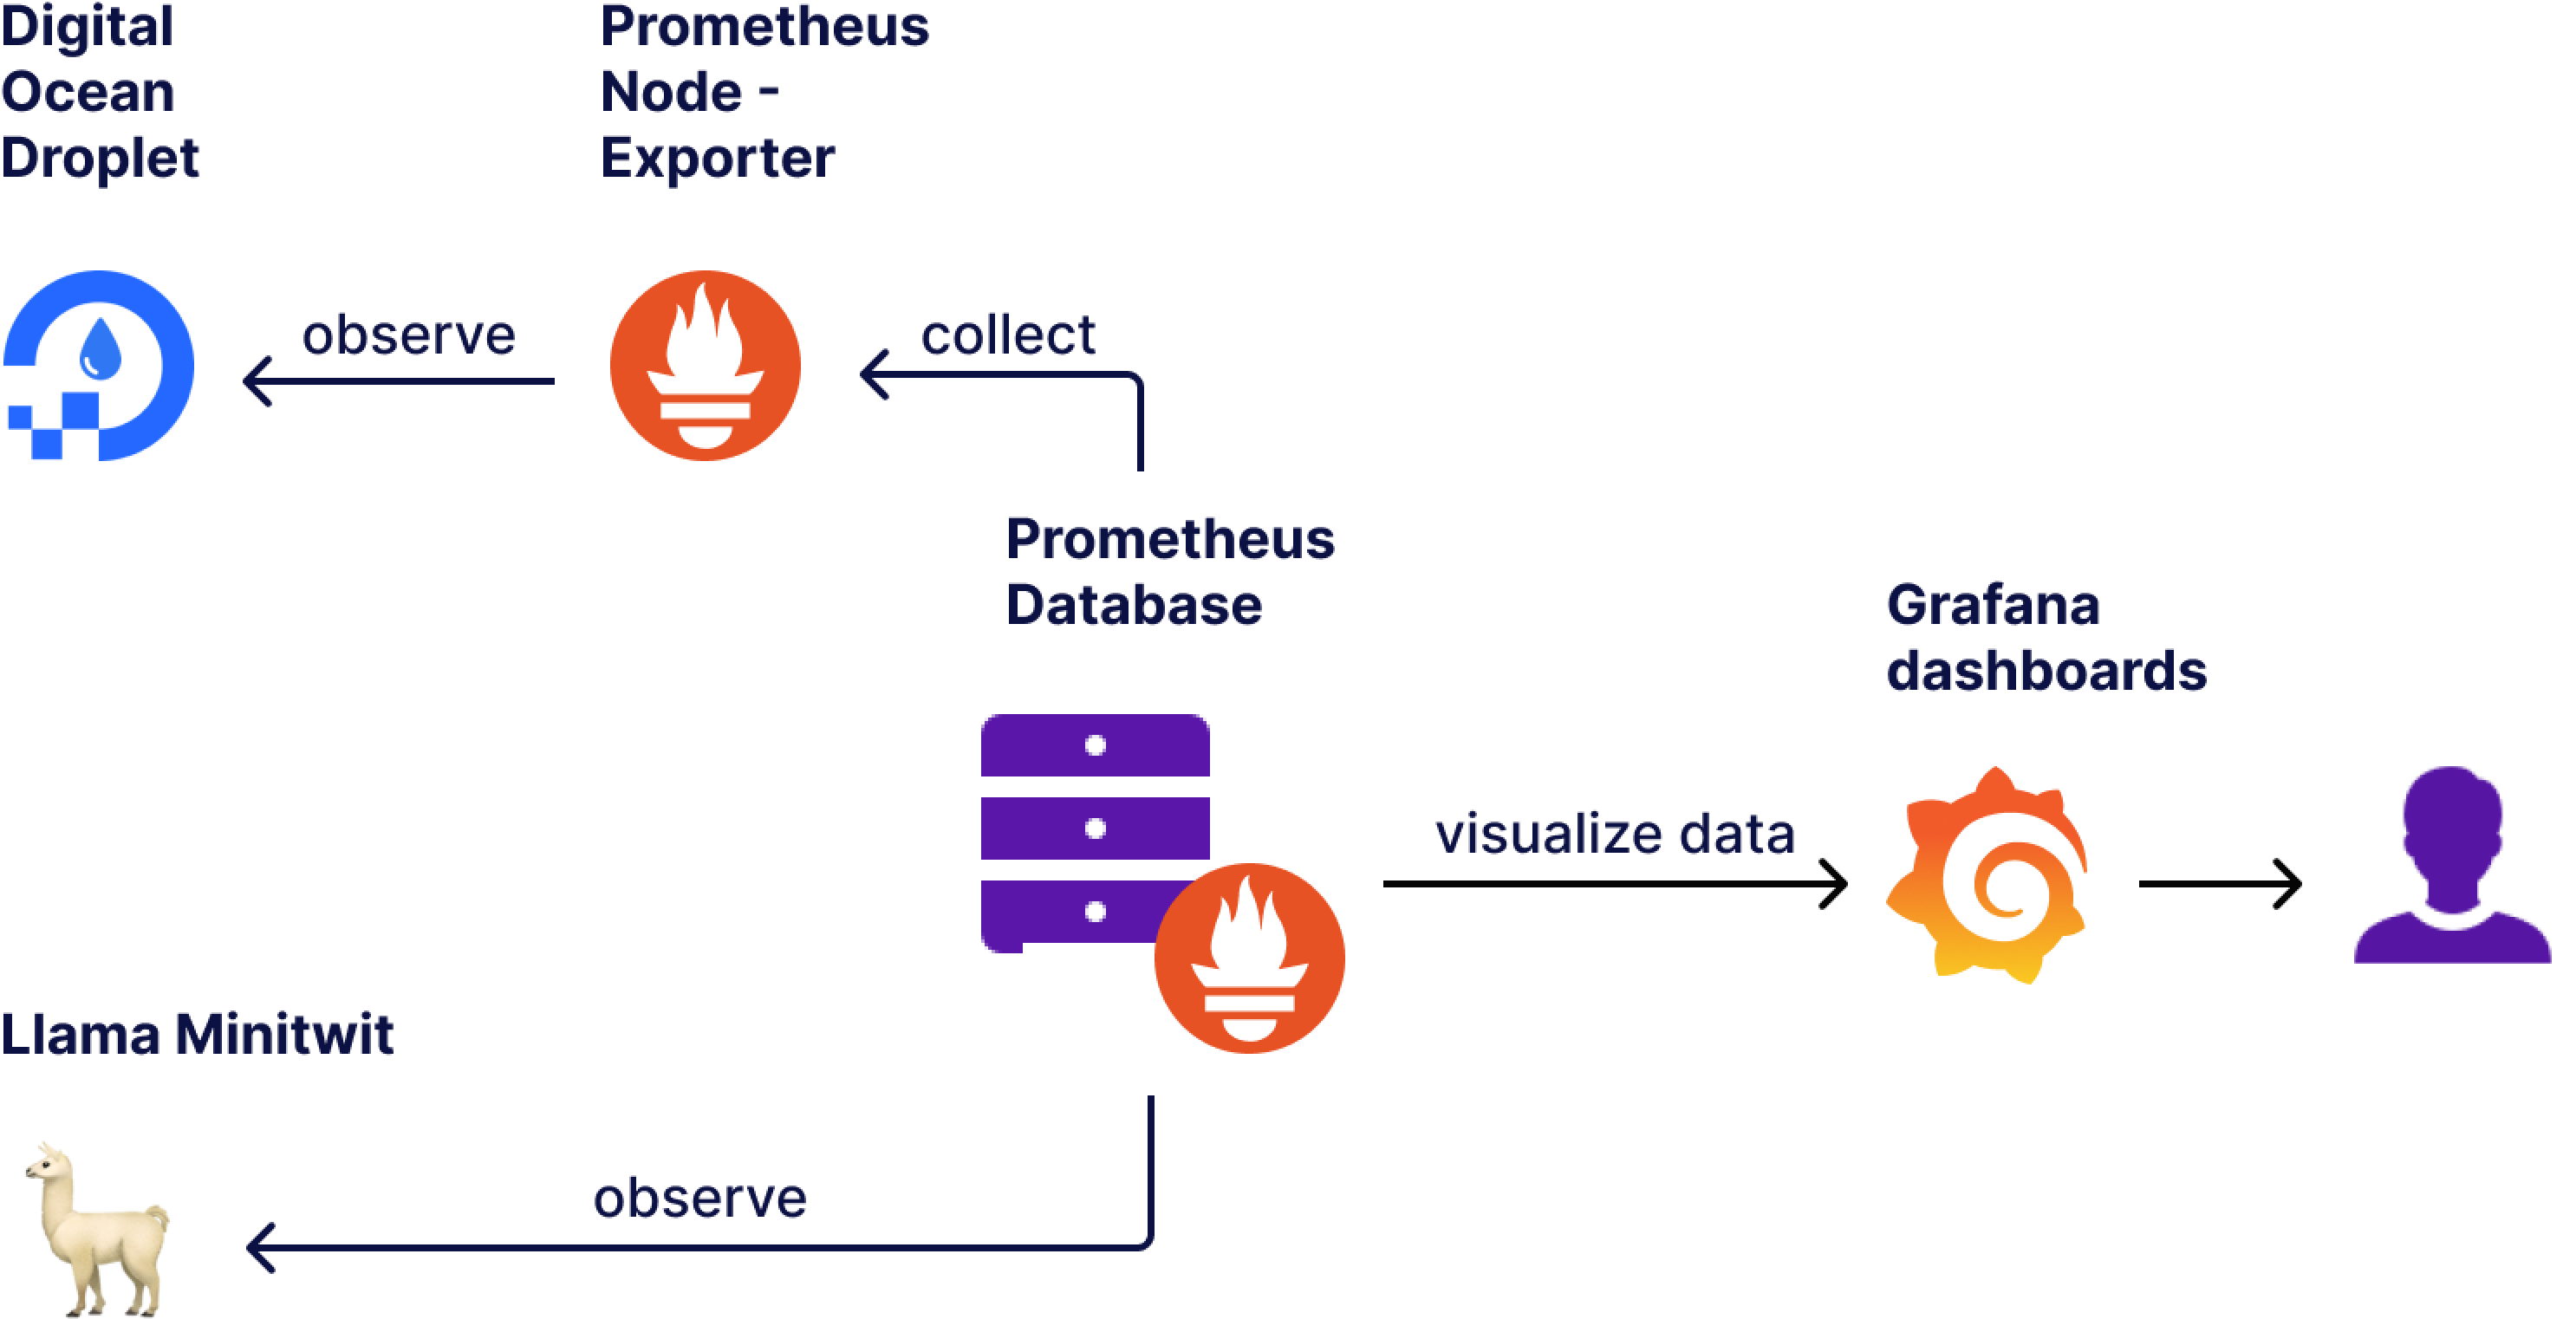
\includegraphics[width=0.7\textwidth]{./images/flow_grafana_prometheus_v2.png} 
    \caption{Visualization flow.}
    \label{fig:visualization_flow}
\end{figure}

Figure \ref{fig:visualization_flow} shows that after data was scraped from our application, it was stored in a Prometheus container and then displayed using Grafana's visualization dashboards. We chose a Grafana and Prometheus stack for multiple reasons:

\begin{enumerate}
    \item These free and open source software (FOSS) helped keep our costs for the overall project low.
    \item They are widely used as industry-standard way of monitoring, have good integration with cloud-origin environments and variety of plugins, provide detailed visualizations and are very user-friendly.
\end{enumerate}

\subsubsection{Active Monitoring}
Despite our existing use of Grafana, we selected the EFK (Elasticsearch, Fluentd, Kibana) stack over Promtail + Loki + Grafana (PLG) for qualitative logging. The EFK stack has a mature ecosystem, well-suited search capabilities, and flexible data processing, which makes it a good choice for our qualitative logging. Figure \ref{fig:efk_stack} presents an overview of our EFK stack architecture.
\\\\
Our Llama-MiniTwit application represents the source of the data we aim to analyze. We utilized Logrus for structured logs within our go application. Fluentd is the log aggregator in this stack. It collects logs from Minitwit, processes them, and forwards them to Elasticsearch. Elasticsearch serves as both a search and analytics engine. It indexes and stores log data forwarded by Fluentd, enabling flexible and fast search capabilities. Kibana is the user interface where we can view and interact with the log data stored in Elasticsearch. The logging stack was initially tested using local Docker containers with various logging scenarios. An example of the log output from the simulator is shown in Figure \ref{fig:kibana_screenshot}.
\begin{figure}[ht]
    \centering
    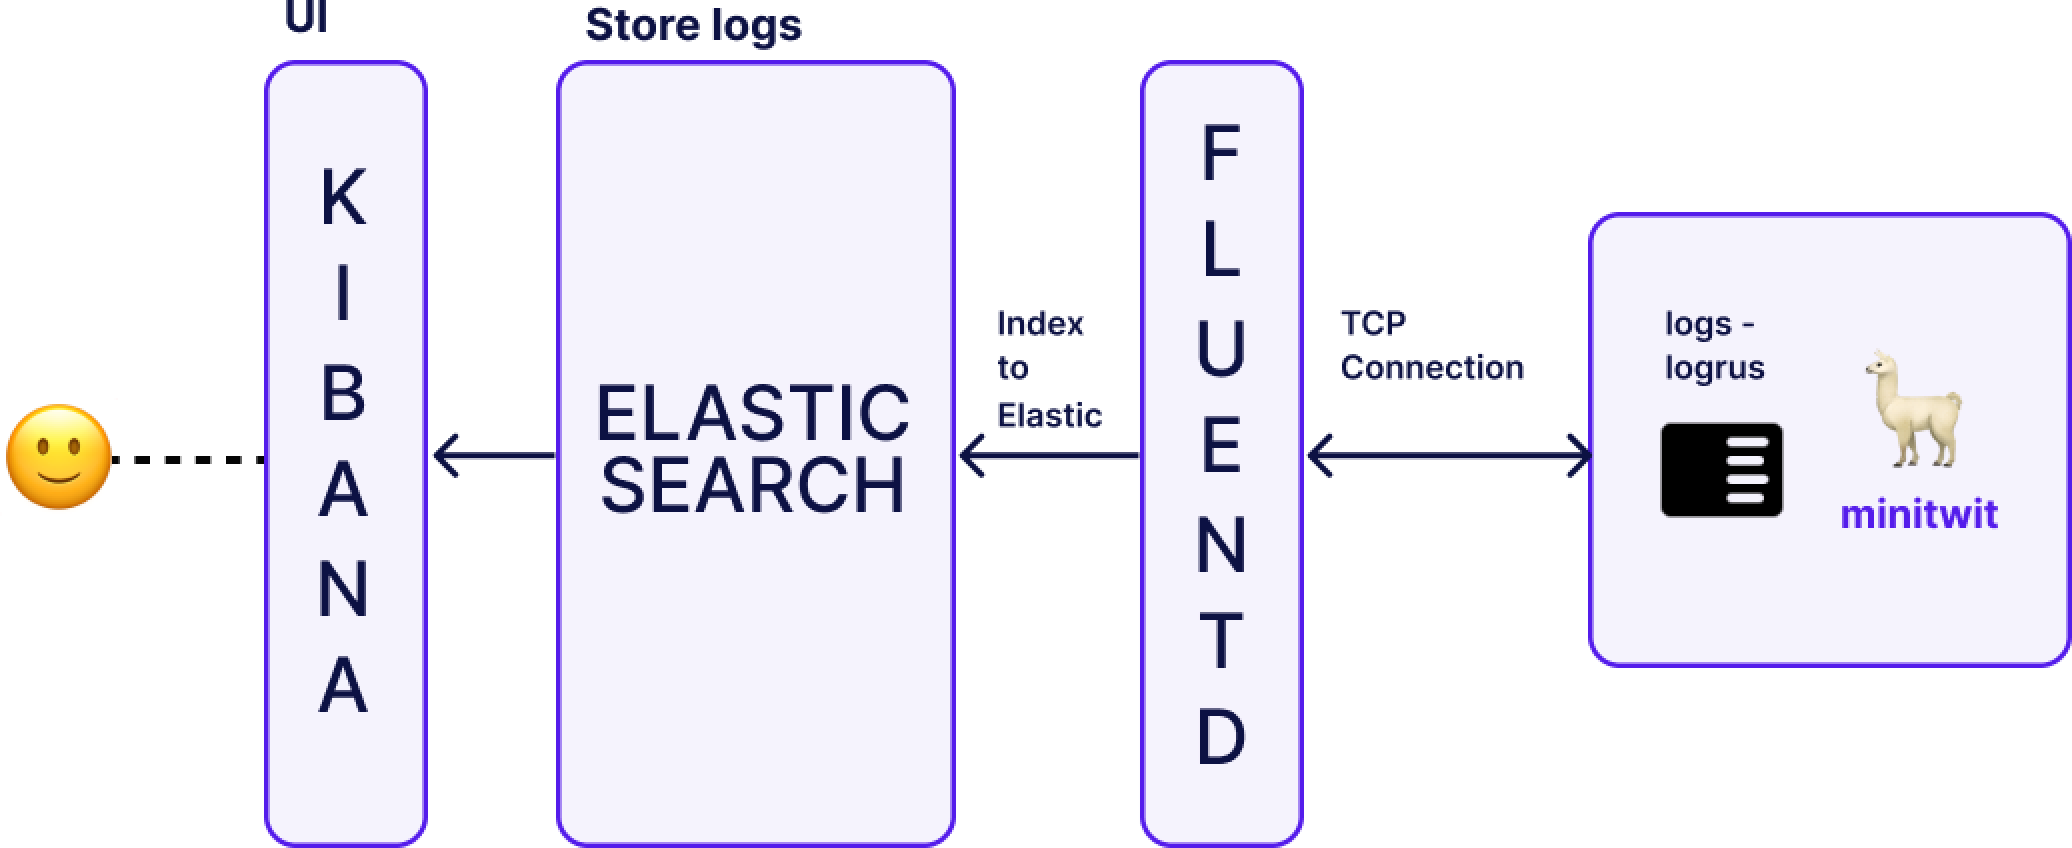
\includegraphics[width=0.8\textwidth]{./images/EFK_stack.png} 
    \caption{EFK Stack Architecture}
    \label{fig:efk_stack}
\end{figure}

\begin{figure}[ht]
    \centering
    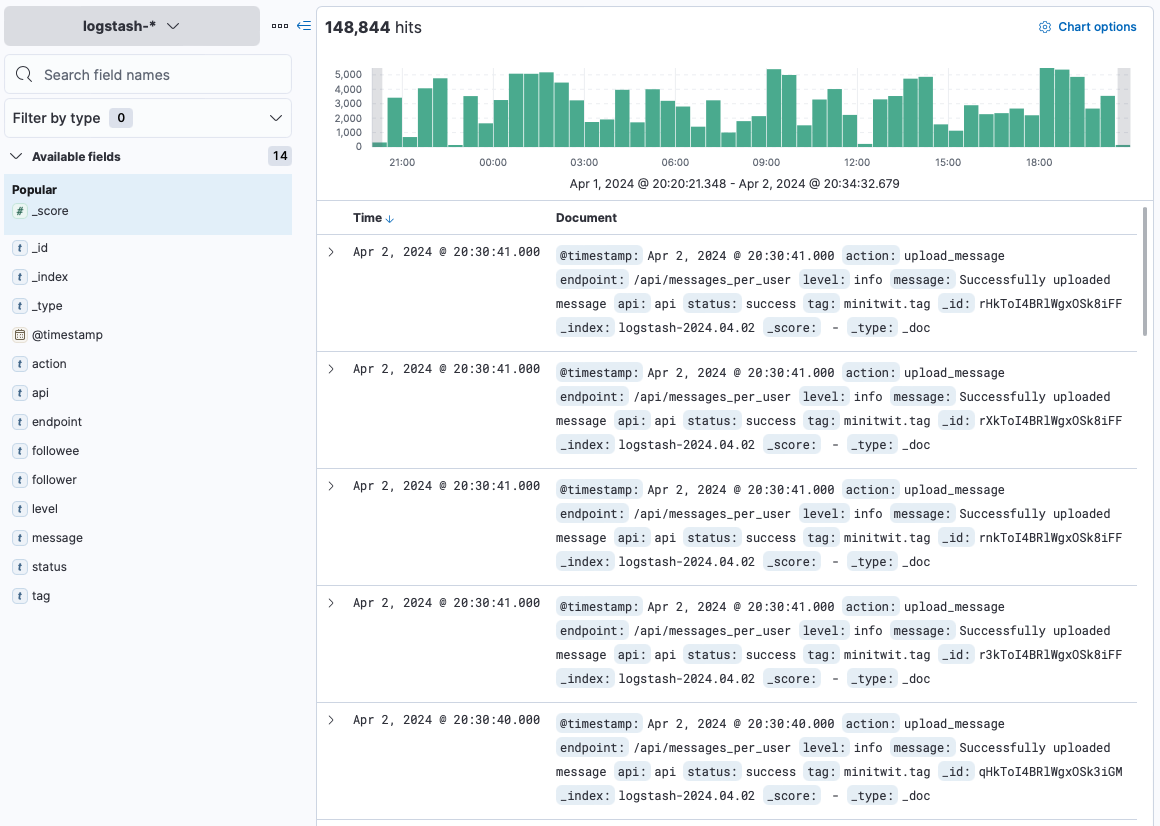
\includegraphics[width=0.7\textwidth]{./images/kibana_screenshot.png} 
    \caption{Logs Generated by the Simulator, Displayed in Kibana}
    \label{fig:kibana_screenshot}
\end{figure}

\subsection{Security Assessment}

\subsubsection{Risk Identification}
The following assets have been identified and considered in the context of the security assessment:

\begin{enumerate}
\item \textbf{User Data}: it includes any information directly connected to users.
\item \textbf{Production VMs}: servers used to run the Llama MiniTwit application.
\item \textbf{Logging Data}: generated logs, especially the qualitative ones.
\item \textbf{Source code}: Llama MiniTwit application source exposition.
\item \textbf{Private Keys and Access Credentials}: keys and credentials used to access parts of the system.
\end{enumerate}

\subsubsection{Risk Scenarios}
\begin{itemize}
\item\textit{\textbf{Risk Scenario 1}}: \textit{Data Breach via SQL Injection} \\
\textbf{Description}: An attacker exploits a SQL injection vulnerability in the Llama MiniTwit application to gain unauthorized access to the database.\\
\textbf{Impact:} Exposure of sensitive user data (emails, passwords, blog posts).\\

\item\textit{\textbf{Risk Scenario 2}}: \textit{Compromised Production VM} \\
\textbf{Description}: The production VM is compromised due to weak SSH credentials, allowing an attacker to gain control over the server.\\
\textbf{Impact:} Unauthorized access to application and data.\\

\item\textit{\textbf{Risk Scenario 3}}: \textit{Distributed Denial of Service (DDoS) Attack} \\
\textbf{Description}: The application is targeted by a DDoS attack, overwhelming the servers and causing service disruption.\\
\textbf{Impact:} Unavailability of the application.\\

\item\textit{\textbf{Risk Scenario 4}}: \textit{White-Box Exploits} \\
\textbf{Description}: The source code of Llama MiniTwit is accidentally made public on a version control platform like GitHub.\\
\textbf{Impact:} Exposure of application vulnerabilities and sensitive information (e.g., hardcoded credentials)\\

\item\textit{\textbf{Risk Scenario 5}}: \textit{Third-Party Software Breach} \\
\textbf{Description}: A third-party software component used in the application is compromised, leading to security vulnerabilities or data breaches.\\
\textbf{Impact:} Software vulnerabilities and data leaks\\

\item\textit{\textbf{Risk Scenario 6}}: \textit{Exposure of Sensitive Information in Logs} \\
\textbf{Description}: Qualitative logs containing sensitive user information and operational details are exposed due to misconfigured logging settings.\\
\textbf{Impact:} Leakage of user behaviour patterns eventually personal information.\\

\item\textit{\textbf{Risk Scenario 7}}: \textit{Brute Force Attack} \\
\textbf{Description}: An attacker that uses trial and error to gain access to passwords, login credentials, and encryption keys.\\
\textbf{Impact:} Unauthorized access to user accounts, data leaks, data manipulation.\\
\end{itemize}

\subsubsection{Risk Analysis and Mitigation}

Below we have determined the severity of each threat and placed them in a risk matrix to prioritize appropriate mitigation strategies. Furthermore, the outcomes are discussed and potential solutions are presented. The severity categories are defined as follows:

\definecolor{lowrisk}{HTML}{88DEBA} 
\definecolor{mediumrisk}{HTML}{FDFC9A} 
\definecolor{highrisk}{HTML}{FDAB9A} 

\begin{table}[h!]
\centering
\small
\arrayrulecolor{black} 
\renewcommand{\arraystretch}{1.5} 
\newcolumntype{a}{>{\columncolor{gray!5}}c}
\begin{tabular}{|c|c|c|c|}
\hline
\rowcolor{white}
& \textbf{Insignificant} & \textbf{Marginal} & \textbf{Critical} \\
\hline
\textbf{Likely} & \cellcolor{mediumrisk} & \cellcolor{highrisk} & \cellcolor{highrisk} \\
\hline
\textbf{Possible} & \cellcolor{lowrisk} & \cellcolor{mediumrisk}  & \cellcolor{highrisk} 1, 5 \\
\hline
\textbf{Unlikely} & \cellcolor{lowrisk} 7 & \cellcolor{lowrisk} 4, 6  & \cellcolor{mediumrisk} 2, 3 \\
\hline
\end{tabular}
\end{table}

\begin{table}[h!]
\centering
\small
\arrayrulecolor{black} 
\renewcommand{\arraystretch}{1.5} 
\newcolumntype{a}{>{\columncolor{gray!5}}c}
\begin{tabular}{|c|c|c|}
\hline
\cellcolor{lowrisk} & Low risk \\
\hline
\cellcolor{mediumrisk} & Medium risk \\
\hline
\cellcolor{highrisk} & High risk \\
\hline
\end{tabular}
\end{table} 

\pagebreak

\textit{\textbf{High Risk}}\vspace{0.2em}
\begin{itemize}
    \item \textbf{1} \textit{Data Breach via SQL Injection:} Our Llama MiniTwit has an abstraction layer in place, so it is highly unlikely to be attacked by a SQL injection. To further mitigate the risk of data loss, regular backups could be implemented.
    \item \textbf{5} \textit{Third-Party Software Breach:} The impact of a third-party software breach can vary. Fortunately, this risk can also be mitigated e.g. checking the security posture, compliance with industry standards, and historical performance.
\end{itemize}

\vspace{0.4em}
\textit{\textbf{Medium Risk}}\vspace{0.2em}
\begin{itemize}
    \item \textbf{2} \textit{Compromised Production VM:} DigitalOcean offers the capability to add a firewall that serves to safeguard access to our virtual machines. However, no additional firewall rules have been implemented to protect the VMs themselves yet.
    \item \textbf{3} \textit{Distributed Denial of Service (DDoS) Attack:} Our application is not that popular, so it is unlikely to be under a DDoS attack. However, it is still possible since our application is public. If such a thing happens it will probably experience some downtime.
\end{itemize}

\vspace{0.4em}
\textit{\textbf{Low Risk}}\vspace{0.2em}
\begin{itemize}
    \item \textbf{4} \textit{White-Box Exploits:} Our Git repository is public, meaning anyone can view our code and potentially create exploits based on it. However, our code review processes provide a layer of protection in such scenarios. Additionally, we have been diligent in ensuring that no credentials are stored in the repository.
    \item \textbf{6} \textit{Exposure of Sensitive Information in Logs:} The implementation of a proxy server plus firewall can render the logs inaccessible from external sources. Even if the logs are accessed by a malicious actor, no behavioural patterns or private user information is being displayed. 
    \item \textbf{7} \textit{Brute Force Attack:} This scenario is unlikely to happen and would only affect one or a few users. Two-factor authentication could be implemented as a potential solution. 
\end{itemize}

\subsubsection{Pen Testing}
We conducted a penetration test using Metasploit and the WMAP plugin. Our main objective was to target the production URL (\texttt{http://134.209.226.165:8081/public}) to identify potential vulnerabilities. The WMAP scan reported no vulnerabilities, as shown in the terminal output below:
\begin{verbatim}
[*] Done.
msf6 > wmap_vulns -l
[*] + [134.209.226.165] (134.209.226.165): directory /log/
[*] 	directory Directory found.
[*] 	GET Res code: 404
[*] + [134.209.226.165] (134.209.226.165): directory /login/
[*] 	directory Directory found.
[*] 	GET Res code: 301
[*] + [134.209.226.165] (134.209.226.165): directory /logout/
[*] 	directory Directory found.
[*] 	GET Res code: 301
[*] + [134.209.226.165] (134.209.226.165): directory /public/
[*] 	directory Directory found.
[*] 	GET Res code: 301
[*] + [134.209.226.165] (134.209.226.165): directory /register/
[*] 	directory Directory found.
[*] 	GET Res code: 301
[*] + [134.209.226.165] (134.209.226.165): directory /static/
[*] 	directory Directory found.
[*] 	GET Res code: 404
[*] + [134.209.226.165] (134.209.226.165): file /login
[*] 	file File found.
[*] 	GET Res code: 200
[*] + [134.209.226.165] (134.209.226.165): file /logout
[*] 	file File found.
[*] 	GET Res code: 302
[*] + [134.209.226.165] (134.209.226.165): file /public
[*] 	file File found.
[*] 	GET Res code: 200
[*] + [134.209.226.165] (134.209.226.165): file /register
[*] 	file File found.
[*] 	GET Res code: 200
msf6 > vulns

Vulnerabilities
===============

Timestamp  Host  Name  References
---------  ----  ----  ----------

msf6 > 
\end{verbatim}


\subsection{Scaling}
Our strategy for scaling mainly relies on the services provided to us by DigitalOcean and our system architecture. Should we need it, we could scale vertically by purchasing droplets with more resources on DigitalOcean. We could also purchase more droplets and create additional swarms around the world. 

\subsection{Our use of AI assistants}
AI-tools such as ChatGPT proved to be very helpful for:
\begin{itemize}
    \item Debugging and handling errors.
    \item How different functions could be implemented in different languages.
\end{itemize}
However, we also found that AI assistants were not helpful for:
\begin{itemize}
    \item Direct translations of code from one language to another.
    \item Providing correct answers for higher complex issues such as adding GORM as database abstraction layer or indexing or database.
\end{itemize}

In general, throughout our project we did not rely heavily on AI assistant as we were able to solve most issues reading documentation and using each other.

\section{Lessons Learned Perspective}
In this section, we describe some of the technical difficulties we ran into during the semester, the lessons we learned from them and reflect on how we these difficulties could have been avoided or how we could have recovered more gracefully.

\subsubsection{Bad Database Management}
Initially, we had successfully running flow that was able to update the docker image, however we were failing to do so because the script which was responsible for rebooting the docker was not running smoothly. as a result we have had a new image, but we were still updating our database with the old one for about two weeks. 
After the script was fixed we were able to reboot our DockerHub and update the Minitwit image with the latest version.

\subsubsection{Resource Starvation}
During the 4th session of the course, we were tasked with deploying our Llama-MiniTwit system to the cloud so that the simulator could eventually interact with it through our API. We partitioned a droplet on DigitalOcean and deployed our app through a Docker container. We had some additional services running on other containers but on the same droplet. Once the simulator started, our Docker container would seemingly randomly be shut down every few hours. After a few weeks, we realized that there was a direct correlation between our container being shut off and a spike in traffic on our Llama-MiniTwit. We realized that the sum of resources we had allocated to each container running on the virtual machine installed on our droplet was higher than the resources we had purchased from Digital Ocean. More specifically, our containers were allowed to consume up to 6GB of RAM, but our droplet only provided us with 4 GB. Thus, when the traffic spiked, the container consumed more RAM than it physically had access to and the OS would kill it.
\\\\

\subsubsection{Slow Llama-MiniTwit}
After the simulator had been running on our live system for a few weeks, we noticed a significant increase in the dataset size, which resulted in much longer query times. To address this issue, we implemented indices in the database using SQL queries. To determine which indices to create, we focused on the processes that were performing the slowest: accessing the public timeline, retrieving messages, and managing followers. For these, we implemented B-tree indices and we managed to optimize the performance of our database queries and ensuring efficient data retrieval.
\\
For user table (unique):
\begin{verbatim}
CREATE INDEX idx_username ON user(username(255));
CREATE INDEX idx_email ON user(email(255));
\end{verbatim}

For message table (non-unique):
\begin{verbatim}
CREATE INDEX idx_author_id ON message(author_id(255));
CREATE INDEX idx_pub_date ON message(pub_date(255));
\end{verbatim}

For follower table:
\begin{verbatim}
CREATE INDEX idx_who_id ON follower(who_id(255));
CREATE INDEX idx_whom_id ON follower(whom_id(255));
\end{verbatim}

\subsection{DevOps Style}

\subsubsection{Good Git Practices}
We established a routine where we worked separately on feature branches, testing our code locally before creating a pull-request to the main branch. To merge into main another developer would then have to review. This greatly reduced the risk of bugs finding their way onto our deployed environment.

\subsubsection{The three DevOps ways}
1) The Principles of Flow
\begin{itemize}
    \item Visibility: We were sharing our work by defining tasks in a Notion board to help us to keep track of what we needed to do.

    \begin{figure}[ht]
        \centering
        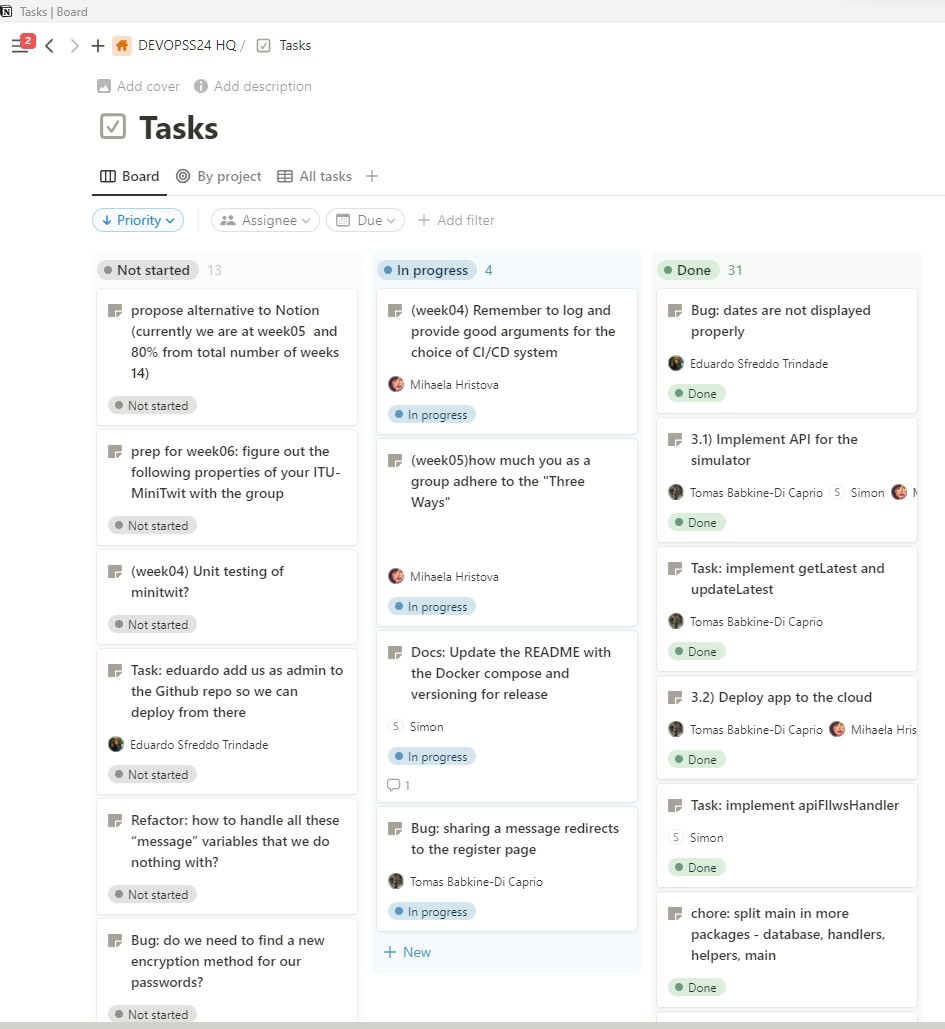
\includegraphics[width=0.8\textwidth]{./images/notion-dashboard-visibility-three-ways.png}
        \caption{Notion dashboard where we keep track of our tasks.}
        \label{fig:notion-dashboard}
    \end{figure}

    \item Limit Work in Progress: We set a limit on the tasks that could be in each column in the Notion board. When we were waiting on a task to be completed, we asked the team member what was causing the delay and helped him/her instead. We made sure to have at least one meeting in person per week.
    
    \item Reduce batch sizes: In our case we looked at each different feature as a single unit operation being refactored, tested and deployed. Instead of implementing all features at once (post messages, follow user, register, etc) we developed and tested one at a time. This shortened the development time significantly and most importantly help us to detect and act on bugs much faster.
\end{itemize}

2) The Principles of Feedback
\begin{itemize}
    \item We tried giving feedback as fast as possible in order to achieve quality, reliability and safety in the technology value stream.
\end{itemize}

3) The Principles of Continual Learning and Experimentation: 
\begin{itemize}
    \item We acknowledged that failure was highly probable at any stage of our process. Thus, we adopted a "no blame culture", where we would discuss occurring problems in order to create a safe work environment.
\end{itemize}

\clearpage
\section{Dependencies}

\subsection*{Application Written in Go}
\begin{itemize}
    \item \textbf{github.com/evalphobia/logrus\_fluent v0.5.4}: a library for logging to Fluentd with Logrus.
    \item \textbf{github.com/gin-gonic/gin v1.9.1}: a HTTP web framework written in Go (Golang).
    \item \textbf{github.com/joho/godotenv v1.5.1}: a Go port of Ruby's dotenv library (loads environment variables from `.env`).
    \item \textbf{github.com/prometheus/client\_golang v1.19.0}: the Prometheus monitoring system and time series database client.
    \item \textbf{github.com/shirou/gopsutil v3.21.11+incompatible}: a library for retrieving system and process metrics (like ps, top).
    \item \textbf{github.com/sirupsen/logrus v1.9.3}: a structured logger for Go (golang), completely API compatible with the standard library logger.
    \item \textbf{gorm.io/driver/sqlite v1.5.5}: GORM SQLite driver.
    \item \textbf{gorm.io/gorm v1.25.7}: The fantastic ORM library for Golang, aims to be developer friendly.
    \item \textbf{github.com/gin-contrib/sessions v0.0.5}: Gin middleware for session management.
    \item \textbf{gorm.io/driver/mysql v1.5.6}: GORM MySQL driver.
\end{itemize}

\subsection*{Python Tests}
\begin{itemize}
    \item \textbf{pymongo==4.7.2}: The Python driver for MongoDB.
    \item \textbf{pytest==8.0.2}: A framework for testing Python code.
    \item \textbf{requests==2.32.2}: Python HTTP for Humans.
    \item \textbf{selenium==4.21.0}: Python bindings for Selenium WebDriver.
\end{itemize}

\subsection*{Third Party Services}
\begin{itemize}
    \item \textbf{nginx}: a web server and reverse proxy server.
    \item \textbf{certbot/certbot:latest}: the latest version of Certbot, a tool for obtaining SSL/TLS certificates from Let's Encrypt.
    \item \textbf{prom/prometheus}: the Prometheus monitoring system and time series database.
    \item \textbf{grafana/grafana:10.2.4}: the latest version of Grafana, an open source platform for monitoring and observability.
    \item \textbf{prom/node-exporter}: Prometheus exporter for hardware and OS metrics exposed by *NIX kernels.
    \item \textbf{fluent/fluentd-kubernetes-daemonset:v1.16.2-debian-elasticsearch7-1.1}: Fluentd Docker image for Kubernetes daemonset with Elasticsearch support.
    \item \textbf{docker.elastic.co/elasticsearch/elasticsearch:7.17.17}: the latest version of Elasticsearch.
    \item \textbf{kibana:7.17.17}: the latest version of Kibana.
\end{itemize}

\clearpage
\section{References}

1. Official website of Go https://go.dev/
-for installation and tutorials

2. LinkedIn learning “Learning Go” by David Gassner
https://www.linkedin.com/learning/learning-go-8399317/explore-go-s-variable-types?u=55937129

3. Reference for indexing the database
https://github.com/dbeaver/dbeaver/wiki/Creating-Indexes

\end{document}